\appendix
\renewcommand\thefigure{\thesection.\arabic{figure}}
\chapter*{Appendix}
\addcontentsline{toc}{chapter}{Appendix}
\setcounter{section}{0}
\renewcommand{\thesection}{\Alph{section}}

%%%%%%%%%%%%%%%%%%%%%%%%%%%%%%%%%%

\section{Damping Factor}\label{damping}

The damping factor plays a crucial role when using RPA calculations to determine the EELS and plasmon eigenmodes. In the theory we mentioned the damping factor $\eta$ (see equations \ref{eq:green_damp} and \ref{eq:pi_damp}), which was shown in the polarisability matrix
\begin{equation}
    \Pi(\mathbf{r}'',\mathbf{r}',\omega) = g_s \lim_{\eta\to 0^+}\sum_{i,j} G(i,j,\omega)\psi_j^\dagger (\mathbf{r}'')\psi_i (\mathbf{r}'')\psi_i^\dagger (\mathbf{r}')\psi_j (\mathbf{r}').
\end{equation}
Based on this definition the damping factor $\eta$ tends to zero when determining the polarisability matrix, however choosing the initial value for $\eta$ can be tricky. In figure \ref{fig:damp_comp} we can see how four different damping factors compare to each other. A damping factor of $\eta=\SI{0.1}{eV}$ is very large, such that certain frequencies which correspond to plasmonic excitations might not be visible on the EELS. A very high damping factor like $\eta=\SI{0.0001}{eV}$ might be better for a good resolution, but it requires determining more frequencies, so that no peaks are left out. Therefore, based on the EELS in figure \ref{fig:damp_comp}, it appears that $\eta=\SI{0.001}{eV}$ is a good damping factor for the RPA calculations. The resolution is better than for $\eta\in\bbrackets{\SI{0.1}{eV},\SI{0.01}{eV}}$ and lower damping factors, like $\eta=\SI{0.0001}{eV}$, do not bring significant changes to the quality of the EELS.

\begin{figure}[H]
    \centering
    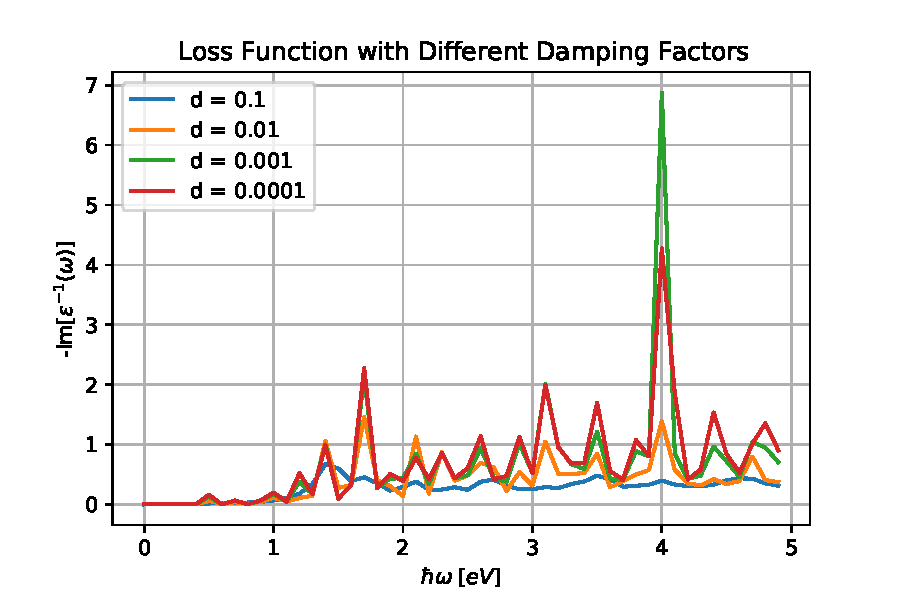
\includegraphics[width=.7\textwidth]{img/eels_damp_comparison.pdf}
    \caption{Comparison of the EELS for a single layer of graphene (snowflake lattice) with four different damping factors $d = \eta$.}
    \label{fig:damp_comp}
\end{figure}



%%%%%%%%%%%%%%%%%%%%%%%%%%%%%%%%

\setcounter{figure}{0}
\section{Figures}\label{figures}

\begin{figure}[H]
    \centering
    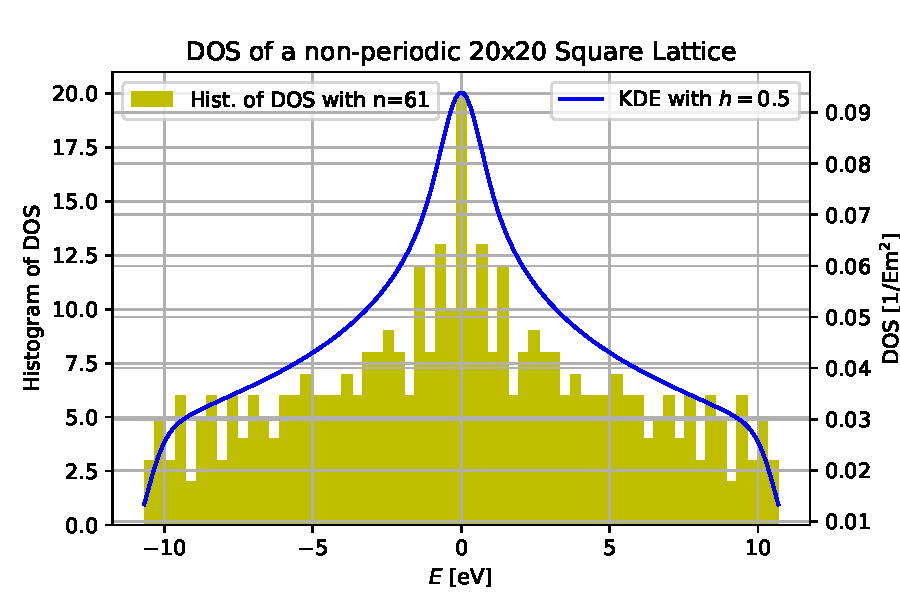
\includegraphics[width=.6\textwidth]{img/DOS_20x20_square_lattice.pdf}
    \caption{Density of states of a $20\times 20$ non-periodic square lattice with different smoothing parameters $h$. The left axis shows the cumulative number of eigenstates $E$ within the total range $[E_{min},E_{max}]$ divided over a certain number of bins (here $n=61$ bins), whereas the right axis corresponds to the KDE of the DOS.}
    \label{fig:DOS_square_lattice}
\end{figure}

\begin{comment}
\begin{figure}[H]
    \centering
    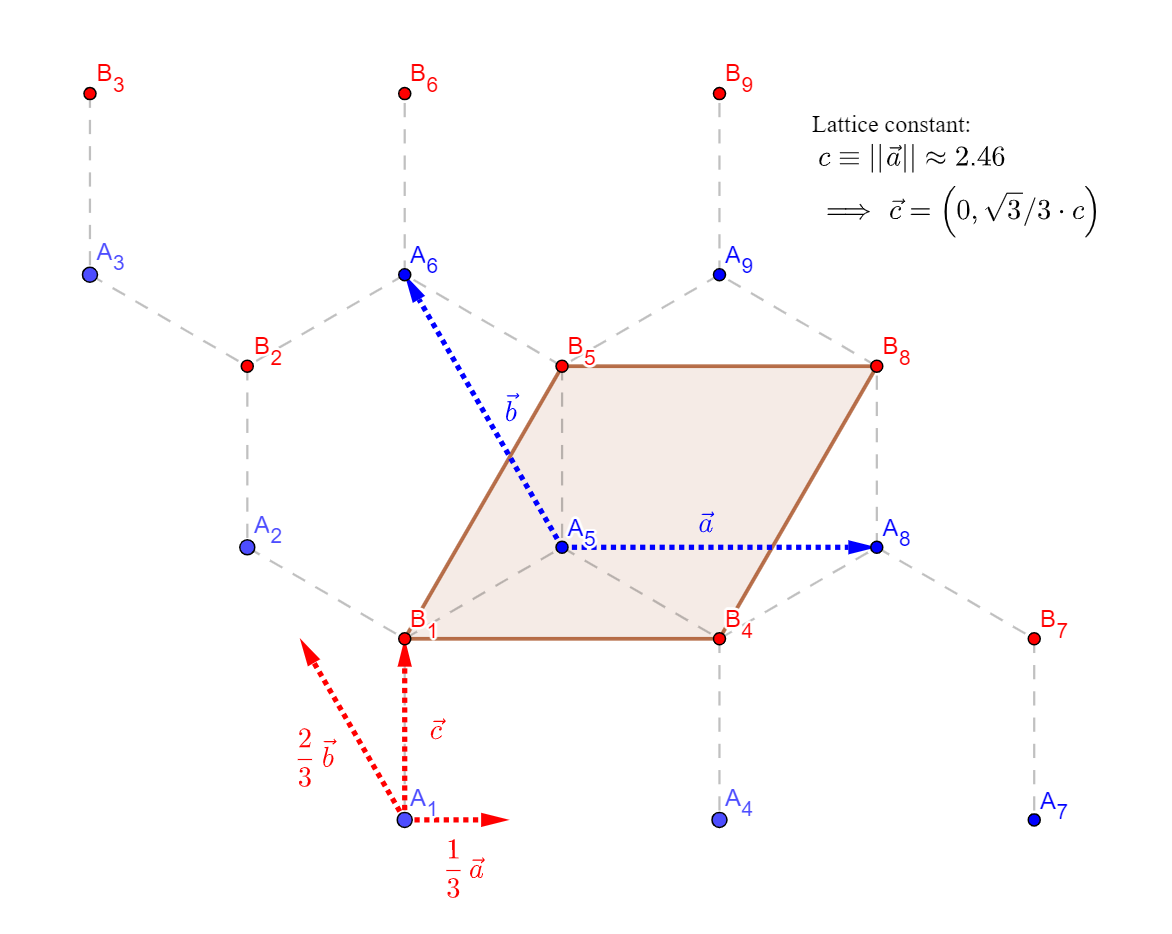
\includegraphics[width=.7\textwidth]{img/graphene_structure_2.PNG}
    \caption{Caption}
    \label{fig:graphene_lattice_2}
\end{figure}
\end{comment}

%%%%%%%%%%%%%%%%%%%%%%%%%%%%%%%%%%%%%%%%%

\setcounter{figure}{0}
\section{Python Algorithms and Code}

For the plots and fits created in this thesis the standard libraries numpy \cite{numpy}, scipy \cite{scipy} and matplotlib \cite{matplotlib} were used. Furthermore for the RPA calculations the algorithms from \textcite{Westerhout2018} were used. The cRPA ab initio calculations were provided by dr. Malte Rösner. For the creation of graphene lattices the package TiPSi (created by Edo van Veen, Guus Slotman, Kaixiang Huang \& Shengjun Yuan) has been used. The documentation for TiPSi can be found under:
\begin{quote}
    \url{http://www.edovanveen.com/tipsi/index.html}.
\end{quote}
For non-linux users (a part of) the package can be downloaded from the Anaconda cloud (provided by Tom Westerhout):
\begin{quote}
    \url{https://anaconda.org/twesterhout/tipsi}
\end{quote}
The source code of the thesis and the figures, can be found in the following repository:
\begin{quote}
    \url{https://github.com/adriansousapoza/Bachelor-Thesis}
\end{quote}
The entire source code used to create the plots, (i.e. determine plasmon eigenmodes, plasmon frequencies, EELS, fitting parameters for the Coulomb interaction, etc.) can be found in the following repository:
\begin{quote}
    \url{https://github.com/adriansousapoza/Bachelor_Plasmons}
\end{quote}
Note that many of these algorithms can only be executed if the user has access to the original data (e.g. ab initio data, h5py files). Last but not least, the algorithms created and used during this internship are based on previous work and ideas from BSc student Samber Bastiaansen and PhD student Tom Westerhout.





